\chapterimage{printing-form} % Chapter heading image

\chapter{Mais sobre Strings e Arrays de Strings}
Bem, vamos voltar um pouco às strings. A seguir, todas as atribuições devem ser entendidas como globais, ou seja, feitas fora de qualquer função, incluindo \textit{main()}.

Indicamos em um capítulo anterior que poderíamos escrever:
\begin{lstlisting}
	char minha_string[40] = "Ted";
\end{lstlisting}
que alocaria espaço para um \textit{array} de 40 bytes e colocaria a string nos primeiros 4 bytes (três para os caracteres entre aspas e um quarto para lidar com a terminação '\textbf{\textbackslash0}').

Na verdade, se tudo o que quiséssemos fazer fosse armazenar o nome ``Ted'', poderíamos escrever:
\begin{lstlisting}
	char meu_nome[] = "Ted";
\end{lstlisting}
e o compilador contaria os caracteres, deixaria espaço para o caractere nulo e armazenaria o total dos quatro caracteres na memória, cuja localização seria retornada pelo nome do \textit{array}, neste caso \textbf{meu\_nome}.

Em algum código, em vez do descrito acima, você verá:
\begin{lstlisting}
	char *meu_nome = "Ted";
\end{lstlisting}
que é uma abordagem alternativa. Existe alguma diferença entre eles? A resposta é... sim. Usando a notação de \textit{array}, 4 bytes de armazenamento no bloco de memória estática são ocupados, um para cada caractere e um para o caractere nulo de terminação. Mas, na notação de ponteiro, os mesmos 4 bytes necessários, mais \textbf{N} bytes para armazenar a variável de ponteiro \textbf{meu\_nome} (onde \textbf{N} depende do sistema, mas geralmente tem um mínimo de 2 bytes e pode ser 4 ou mais). Veja a Figura \ref{fig:arrayponteiro}.

\begin{figure}[ht]
	\begin{center}
		% Graphic for TeX using PGF
% Title: /home/araujo/Dropbox/VerbTeX/LivroComputadores/Pictures/memoria.dia
% Creator: Dia v0.97.3
% CreationDate: Sun May 21 11:59:17 2017
% For: araujo
% \usepackage{tikz}
% The following commands are not supported in PSTricks at present
% We define them conditionally, so when they are implemented,
% this pgf file will use them.
\ifx\du\undefined
  \newlength{\du}
\fi
\setlength{\du}{15\unitlength}

\begin{tikzpicture}
\pgftransformxscale{1.000000}
\pgftransformyscale{-1.000000}
\definecolor{dialinecolor}{rgb}{0.000000, 0.000000, 0.000000}
\pgfsetstrokecolor{dialinecolor}
\definecolor{dialinecolor}{rgb}{1.000000, 1.000000, 1.000000}
\pgfsetfillcolor{dialinecolor}

%cabeçalho
\node[anchor=west] at (21.3\du,7.5\du) {Endere\c{c}o};
\node[anchor=west] at (24.4\du,6.002347\du){Mem\'{o}ria};
\node[anchor=west] at (27.3\du,7.5\du){Array};

%conteúdo
\node[anchor=west] at (25.6\du,6.600000\du){.};
\node[anchor=west] at (25.6\du,7.000000\du){.};
\node[anchor=west] at (25.6\du,7.600000\du){.};
\node at (26\du,8.8\du) {'T'};
\node at (26\du,10.2\du){'e'};
\node at (26\du,11.6\du){'d'};
\node at (26\du,13\du)  {'\textbackslash0'};
\node[anchor=west] at (25.6\du,19.6\du){.};
\node[anchor=west] at (25.6\du,20\du){.};
\node[anchor=west] at (25.6\du,20.6\du){.};

%retângulos
\draw (25\du,6.6\du)--(25\du,8.0\du)--(27\du,8\du)--(27\du,6.6\du);
\draw (25\du,8.0\du)--(25\du,9.4\du)--(27\du,9.4\du)--(27\du,8\du);
\draw (25\du,9.4\du)--(25\du,10.8\du)--(27\du,10.8\du)--(27.\du,9.4\du);
\draw (25\du,10.8\du)--(25\du,12.2\du)--(27\du,12.2\du)--(27.\du,10.8\du);
\draw (25\du,12.2\du)--(25\du,13.6\du)--(27\du,13.6\du)--(27.\du,12.2\du);
\draw (25\du,13.6\du)--(25\du,15\du)--(27\du,15\du)--(27.\du,13.6\du);
\draw (25\du,15\du)--(25\du,16.4\du)--(27\du,16.4\du)--(27.\du,15\du);
\draw (25\du,16.4\du)--(25\du,17.8\du)--(27\du,17.8\du)--(27.\du,16.4\du);
\draw (25\du,17.8\du)--(25\du,19.2\du)--(27\du,19.2\du)--(27.\du,17.8\du);
\draw (25\du,19.2\du)--(25\du,20.6\du);
\draw (27\du,19.2\du)--(27\du,20.6\du);

%endereços
\node[anchor=west] at (21\du,8.8\du) {0x5a691010};
\node[anchor=west] at (21\du,10.2\du){0x5a691011};
\node[anchor=west] at (21\du,11.6\du){0x5a691012};
\node[anchor=west] at (21\du,13\du)  {0x5a691013};
\node[anchor=west] at (21\du,14.4\du){0x5a691014};
\node[anchor=west] at (21\du,15.8\du){0x5a691015};
\node[anchor=west] at (21\du,17.2\du){0x5a691016};
\node[anchor=west] at (21\du,18.4\du){0x5a691017};

% variáveis
\node[anchor=west] at (27.3\du,8.8\du){meu\_array};

%ponteiro
%cabeçalho
\node[anchor=west] at (33.3\du,7.5\du) {Endere\c{c}o};
\node[anchor=west] at (36.4\du,6.002347\du){Mem\'{o}ria};
\node[anchor=west] at (39.3\du,7.57\du){Ponteiro};

%conteúdo
\node[anchor=west] at (37.6\du,6.600000\du){.};
\node[anchor=west] at (37.6\du,7.000000\du){.};
\node[anchor=west] at (37.6\du,7.600000\du){.};
\node at (38\du,8.8\du) {'T'};
\node at (38\du,10.2\du){'e'};
\node at (38\du,11.6\du){'d'};
\node at (38\du,13\du)  {'\textbackslash0'};
\node at (38\du,14.4\du) {10};
\node at (38\du,15.8\du) {10};
\node at (38\du,17.2\du) {69};
\node at (38\du,18.6\du) {5a};
\node[anchor=west] at (37.6\du,19.6\du){.};
\node[anchor=west] at (37.6\du,20\du){.};
\node[anchor=west] at (37.6\du,20.6\du){.};

%retângulos
\draw (37\du,6.6\du)--(37\du,8.0\du)--(39\du,8\du)--(39\du,6.6\du);
\draw (37\du,8.0\du)--(37\du,9.4\du)--(39\du,9.4\du)--(39\du,8\du);
\draw (37\du,9.4\du)--(37\du,10.8\du)--(39\du,10.8\du)--(39.\du,9.4\du);
\draw (37\du,10.8\du)--(37\du,12.2\du)--(39\du,12.2\du)--(39.\du,10.8\du);
\draw (37\du,12.2\du)--(37\du,13.6\du)--(39\du,13.6\du)--(39.\du,12.2\du);
\draw (37\du,13.6\du)--(37\du,15\du)--(39\du,15\du)--(39.\du,13.6\du);
\draw (37\du,15\du)--(37\du,16.4\du)--(39\du,16.4\du)--(39.\du,15\du);
\draw (37\du,16.4\du)--(37\du,17.8\du)--(39\du,17.8\du)--(39.\du,16.4\du);
\draw (37\du,17.8\du)--(37\du,19.2\du)--(39\du,19.2\du)--(39.\du,17.8\du);
\draw (37\du,19.2\du)--(37\du,20.6\du);
\draw (39\du,19.2\du)--(39\du,20.6\du);

%endereços
\node[anchor=west] at (33\du,8.8\du) {0x5a691010};
\node[anchor=west] at (33\du,10.2\du){0x5a691011};
\node[anchor=west] at (33\du,11.6\du){0x5a691012};
\node[anchor=west] at (33\du,13\du)  {0x5a691013};
\node[anchor=west] at (33\du,14.4\du){0x5a691014};
\node[anchor=west] at (33\du,15.8\du){0x5a691015};
\node[anchor=west] at (33\du,17.2\du){0x5a691016};
\node[anchor=west] at (33\du,18.4\du){0x5a691017};

% variáveis
\node[anchor=west] at (39.3\du,8.8\du){*meu\_array};
\node[anchor=west] at (39.4\du,16.4\du){meu\_array};

\draw [decorate, ultra thick,
decoration = {calligraphic brace}] (39.3\du,13.6\du) --  (39.3\du,19.2\du);

\end{tikzpicture}

		\caption{Uso da memória com Array e Ponteiro (cada posição 1 byte).}
		\label{fig:arrayponteiro}
	\end{center}
	\label{enderecos}
\end{figure}

Na notação de \textit{array}, \textbf{meu\_nome} é a abreviação de \textbf{\&meu\_nome[0]}, que é o endereço do primeiro elemento do \textit{array}. Como a localização do \textit{array} é fixada durante o tempo de execução, isso é uma constante (não uma variável). Na notação de ponteiro, \textbf{meu\_nome} é uma variável. Quanto a qual é o \textbf{melhor} método, isso depende do que você vai fazer no resto do programa.

Vamos agora dar um passo adiante e considerar o que acontece se cada uma dessas declarações for feita dentro de uma função, em oposição a globalmente fora dos limites de qualquer função.

\begin{lstlisting}
	void minha_funcao_A(char *ptr)
		{
		char a[] = "ABCDE";
		.
		.
		}
		
	void minha_funcao_B(char *ptr)
		{
		char *cp = "FGHIJ";
		.
		.
		}
\end{lstlisting}

No caso de \textbf{minha\_funcao\_A}, o conteúdo, ou valor(es) do \textit{array} \textbf{a[]} é considerado como sendo os dados. Diz-se que o \textit{array} foi inicializado com os valores \textbf{ABCDE}. No caso de \textbf{minha\_funcao\_B}, o valor do ponteiro \textbf{cp} é considerado como sendo o dado. O ponteiro foi inicializado para apontar para a string \textbf{FGHIJ}. Tanto em \textbf{minha\_funcao\_A} quanto em \textbf{minha\_funcao\_B} as definições são variáveis locais e, portanto, a string \textbf{ABCDE} é armazenada na pilha, assim como o valor do ponteiro \textbf{cp}. A string \textbf{FGHIJ} pode ser armazenada em qualquer lugar. No meu sistema, ele fica armazenado no segmento de dados, também conhecido como \textit{heap}. Nas Figuras \ref{fig:memarray} e \ref{fig:mempointer} podemos ver como esses elementos são alocados na pilha (stack) ou na memória de dados (heap) conforme a forma de sua declaração.

\begin{figure}[ht]
	\begin{center}
		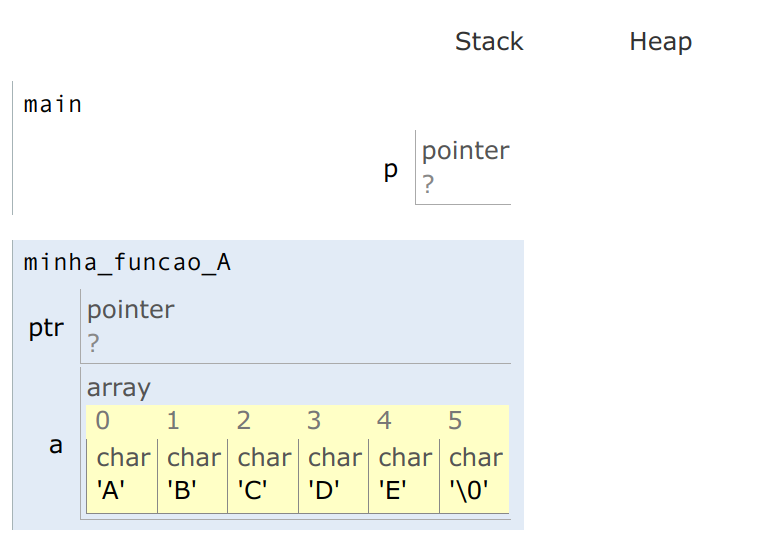
\includegraphics[width=0.5\textwidth]{Pictures/memarray}
		\caption{Declaração de string com Array.}
		\label{fig:memarray}
	\end{center}
\end{figure}

\begin{figure}[ht]
	\begin{center}
		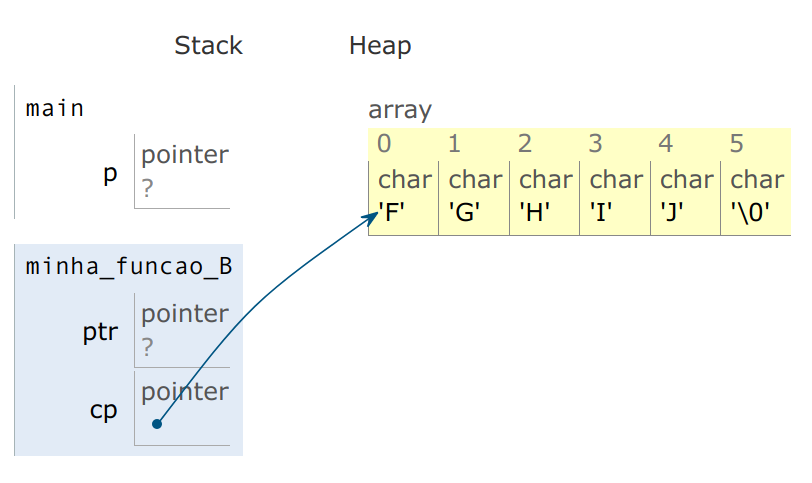
\includegraphics[width=0.5\textwidth]{Pictures/mempointer}
		\caption{Declaração de string com Ponteiro.}
		\label{fig:mempointer}
	\end{center}
\end{figure}

A propósito, a inicialização do \textit{array} de variáveis automáticas como fiz em \textbf{minha\_funcao\_A} era ilegal no livro \textit{K\&R} C antigo e apenas ``atingiu a maioridade'' a partir do ANSI C. Um fato que pode ser importante quando se considera portabilidade e compatibilidade com versões anteriores.

Já que estamos discutindo o relacionamento/diferenças entre ponteiros e \textit{arrays}, vamos prosseguir para os \textit{arrays} multidimensionais. Considere, por exemplo, o \textit{array}:
\begin{lstlisting}
	char multi[5][10];
\end{lstlisting}

O que isso significa? Bem, vamos considerar uma declaração com a seguinte configuração:\\  	char \underline{multi[5]}[10];

Vamos considerar a parte sublinhada como o ``nome'' de um \textit{array}. Depois, acrescentando \textbf{char} e o \textbf{[10]}, temos um \textit{array} de 10 caracteres. Mas, o próprio nome \textbf{multi[5]} é um \textit{array} que indica que existem 5 elementos, cada um sendo um \textit{array} de 10 caracteres. Portanto, temos um \textit{array} de 5 \textit{arrays} de 10 caracteres cada.

Suponha que preenchemos este \textit{array} bidimensional com algum tipo de dado. Na memória, pode parecer que foi formado pela inicialização de 5 \textit{arrays} separados usando algo como:
\begin{lstlisting}
	multi[0] = {'0','1','2','3','4','5','6','7','8','9'}
	multi[1] = {'a','b','c','d','e','f','g','h','i','j'}
	multi[2] = {'A','B','C','D','E','F','G','H','I','J'}
	multi[3] = {'9','8','7','6','5','4','3','2','1','0'}
	multi[4] = {'J','I','H','G','F','E','D','C','B','A'}
\end{lstlisting}

Ao mesmo tempo, elementos individuais podem ser endereçados usando uma sintaxe como:
\begin{lstlisting}
	multi[0][3] = '3'
	multi[1][7] = 'h'
	multi[4][0] = 'J'
\end{lstlisting}

Como os \textit{arrays} são contíguos na memória, nosso bloco de memória real para o caso acima deve ser semelhante a:

\vspace{1em}
\ifx\du\undefined
\newlength{\du}
\fi
\setlength{\du}{15\unitlength}
\begin{tikzpicture}
\pgftransformxscale{1.000000}
\pgftransformyscale{-1.000000}
\definecolor{dialinecolor}{rgb}{0.000000, 0.000000, 0.000000}
\pgfsetstrokecolor{dialinecolor}
\definecolor{dialinecolor}{rgb}{1.000000, 1.000000, 1.000000}
\pgfsetfillcolor{dialinecolor}

\node at (3\du,0\du){0123456789abcdefghijABCDEFGHIJ9876543210JIHGFEDCBA};
\draw[->] (-4.6\du, 2\du) arc (90:175:1);
\node at (1.1\du, 2\du){começando no endereço \&multi[0][0]};
\end{tikzpicture}

Observe que eu não escrevi \textbf{multi[0] = "0123456789"}. Se eu tivesse feito isso, uma terminação `\textbf{\textbackslash0}' estaria implícita, pois sempre que as aspas duplas são usadas, um caractere `\textbf{\textbackslash0}' é anexado aos caracteres contidos nessas aspas. Se fosse esse o caso, eu teria que reservar um espaço para 11 caracteres por linha em vez de 10.

Meu objetivo aqui é ilustrar como a memória é configurada para \textit{arrays} bidimensionais. Ou seja, este é um \textit{array} bidimensional de caracteres, NÃO um \textit{array} de ``strings''.

Agora, o compilador sabe quantas colunas estão presentes no \textit{array} para que possa interpretar \textbf{multi + 1} como o endereço do `a' na 2ª linha. Ou seja, ele adiciona 10, o número de colunas, para obter essa localização. Se estivéssemos lidando com inteiros e um \textit{array} com a mesma dimensão, o compilador adicionaria \textbf{10 * sizeof(int)} que, na minha máquina, seria 40.
Assim, o endereço do 9 na 4ª linha acima seria \&multi[3][0] ou *(multi + 3) em notação de ponteiros. Para obter o conteúdo do 2º elemento na 4ª linha, adicionamos 1 a este endereço e desreferenciamos o resultado como em
\begin{lstlisting}
	*(*(multi + 3) + 1)
\end{lstlisting}

Com um pouco de reflexão, podemos ver que:
\begin{lstlisting}
	*(*(multi + row) + col) e
	multi[row][col] levam aos mesmo resultado.
\end{lstlisting}

O programa a seguir ilustra isso usando \textit{arrays} de inteiros em vez de \textit{arrays} de caracteres.

\lstinputlisting[label={prog6-1}, caption={Array bidimensional e ponteiros}, numbers=left, numberstyle=\tiny, stepnumber=1]{code/prog6-1.c}

Por causa da dupla desreferência necessária na versão do ponteiro, o nome de um \textit{array} bidimensional é frequentemente considerado equivalente a um ponteiro para um ponteiro. Com um \textit{array} tridimensional estaríamos lidando com um \textit{array} de \textit{arrays} de \textit{arrays} e alguns podem dizer que seu nome seria equivalente a um ponteiro para um ponteiro para um ponteiro. No entanto, aqui inicialmente reservamos o bloco de memória para o \textit{array}, definindo-o usando a notação de \textit{array}. Portanto, estamos lidando com uma constante, não uma variável. Ou seja, estamos falando de um endereço fixo, não de um ponteiro variável. A função de desreferenciação usada acima nos permite acessar qualquer elemento no \textit{array} de \textit{arrays} sem a necessidade de alterar o valor desse endereço (o endereço de \textbf{multi[0][0]} conforme fornecido pelo símbolo \textbf{multi}).
